\chapter{Описание существующих решений}

\section{Python}

Python \cite{python} --- интерпретируемый язык программирования с сильной динамической типизацией. Официально язык был представлен в 1991 году. Существует множество реализаций интерпретатора языка Python \cite{juthon} \cite{ironpython} \cite{pypy}. Среди них канонической считается реализация CPython, разработанная на языке C и официально представленная в 1994 году. \cite{cpython}

Интерпретатор CPython использует механизм GIL (Global Interpreter Lock, глобальная блокировка интерпретатора), который обеспечивает однопоточное выполнение байт-кода Python. Этот механизм упрощает реализацию CPython, делая объектную модель (включая встроенные типы, такие как dict) неявно защищённой от конкурентного доступа и упрощая многопоточное выполнение программ. Однако некоторые модули расширения (как стандартные, так и сторонние) \cite{python_extensions} освобождают GIL при выполнении ресурсоёмких задач, таких как сжатие или хеширование. Кроме того, GIL всегда освобождается при выполнении ввода-вывода. \cite{gil}

\subsection{Выделение памяти}

Все объекты программы на языке Python размещаются в \textbf{приватной куче} (private heap), управление которой обеспечивается встроенным в интерпретатор диспетчером памяти. \cite{python_memory}

На самом низком уровне распределитель необработанной памяти (raw memory allocator) взаимодействует с диспетчером памяти операционной системы и гарантирует, что в приватной куче есть достаточно места для хранения всех данных, используемых программой. Помимо распределителя необработанной памяти используется несколько объектно-ориентированных распределителей, которые реализуют различные политики управления памятью, адаптированные к особенностям каждого типа данных. Диспетчер памяти Python делегирует часть работы объектно-ориентированным аллокаторам, гарантируя, что они работают в пределах приватной кучи. \cite{python_memory}

Для выделения памяти допускается использование как функций API Python/C, так и функций стандартной библиотеки языка C. В большинстве ситуаций рекомендуется выделять память в приватной куче, чтобы интерпретатор Python имел более точное представление об использовании памяти. \cite{python_memory}

Все функции распределения памяти в языке Python принадлежат одному из трёх \textbf{доменов} (PyMemAllocatorDomain). Эти домены представляют разные стратегии распределения и оптимизированы для разных целей. \cite{python_memory}

\begin{enumerate}[label*=\arabic*.]
	\item \textbf{Raw domain} предназначен для выделения памяти для буферов общего назначения, где выделение должно передаваться системному аллокатору или где аллокатор может работать без GIL. Память запрашивается непосредственно у операционной системы.
	\item \textbf{<<Mem>> domain} предназначен для выделения памяти для буферов Python и буферов общего назначения, где выделение должно выполняться с удержанием GIL. Память берётся из приватной кучи Python.
	\item \textbf{Object domain} предназначен для выделения памяти для объектов Python. Память берётся из приватной кучи Python.
\end{enumerate}

При освобождении памяти, ранее выделенной функциями, принадлежащими какому-либо домену, необходимо использовать соответствующие функции освобождения из того же домена. \cite{python_memory}



\subsection{Структура объекта}

Основной алгоритм сборки мусора, используемый CPython, --- подсчет ссылок. Для его реализации в структуре объекта Python предусмотрены поля, хранящие число ссылок и данные о типе объекта (\textbf{PyObject\_HEAD}), а также указатели на элементы двусвязного списка объектов, отслеживаемых сборщиком мусора (\textbf{PyGC\_Head}). Структура объекта Python представлена на рисунке \ref{fig:pyobject}.~\cite{python_gc}

\begin{figure}[H]
	\centering
	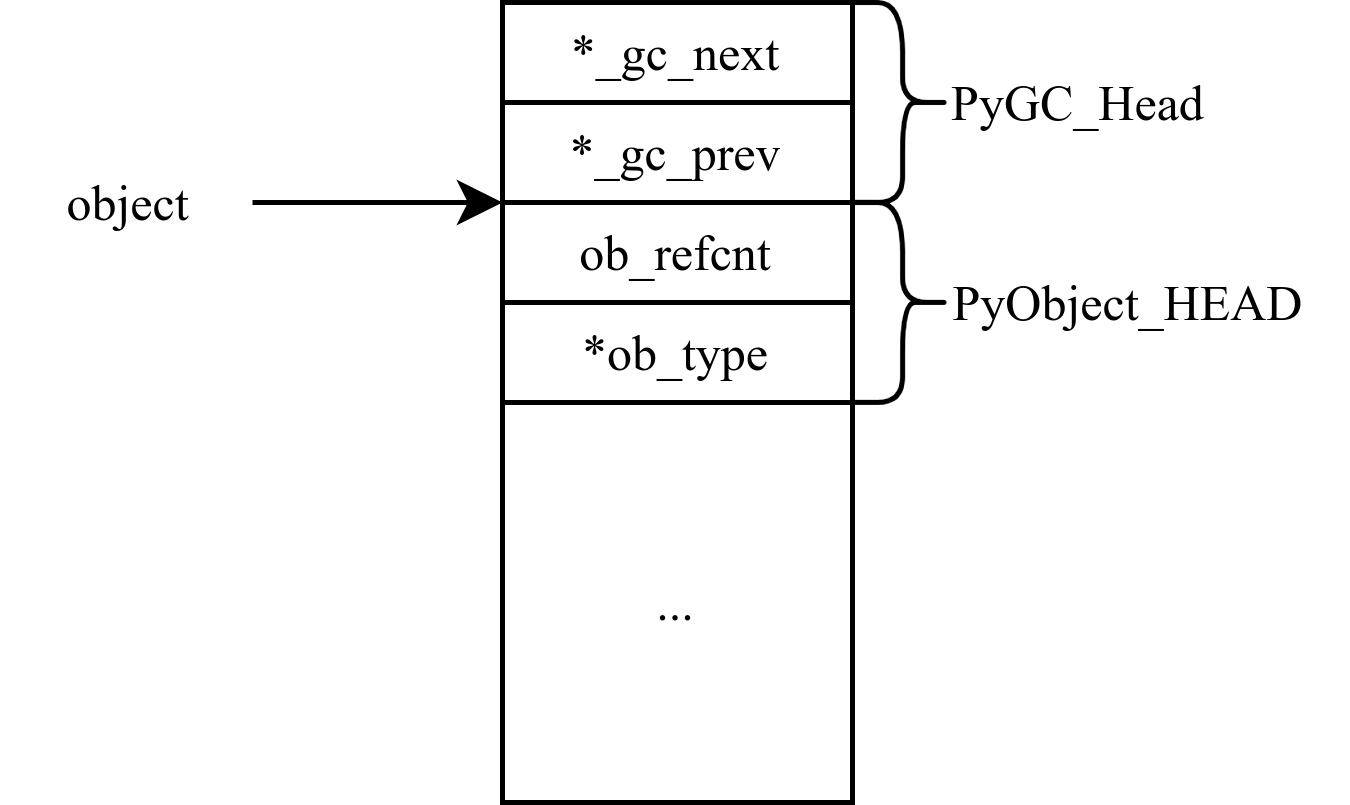
\includegraphics[scale=0.27]{assets/python-object.png}
	\caption{Структура объекта Python}
	\label{fig:pyobject}
\end{figure}

Когда необходима дополнительная информация, связанная со сборщиком мусора, к полям PyGC\_Head можно получить доступ с помощью адресной арифметики и приведения типа исходного объекта. \cite{python_gc}

Двусвязные списки используются по той причине, что они эффективно поддерживают операции, наиболее часто используемые при выполнении алгоритма сбора мусора, такие как перемещение объекта из одного раздела в другой, добавление нового объекта, полное удаление объекта, а также разбиение и объединение списков. \cite{python_gc}



\subsection{Сборка мусора}

Основная проблема подсчета ссылок заключается в том, что он не обрабатывает циклические ссылки. Для её решения используется отдельный сборщик мусора, который занимается только очисткой объектов-контейнеров, то есть объектов, которые могут содержать ссылки на другие объекты. \cite{python_gc}

На рисунках \ref{fig:python-gc} и \ref{fig:python-free} представлены схемы алгоритмов сборки мусора, которые обрабатывают циклические ссылки. \cite{python_gc}

\begin{figure}[H]
	\centering
	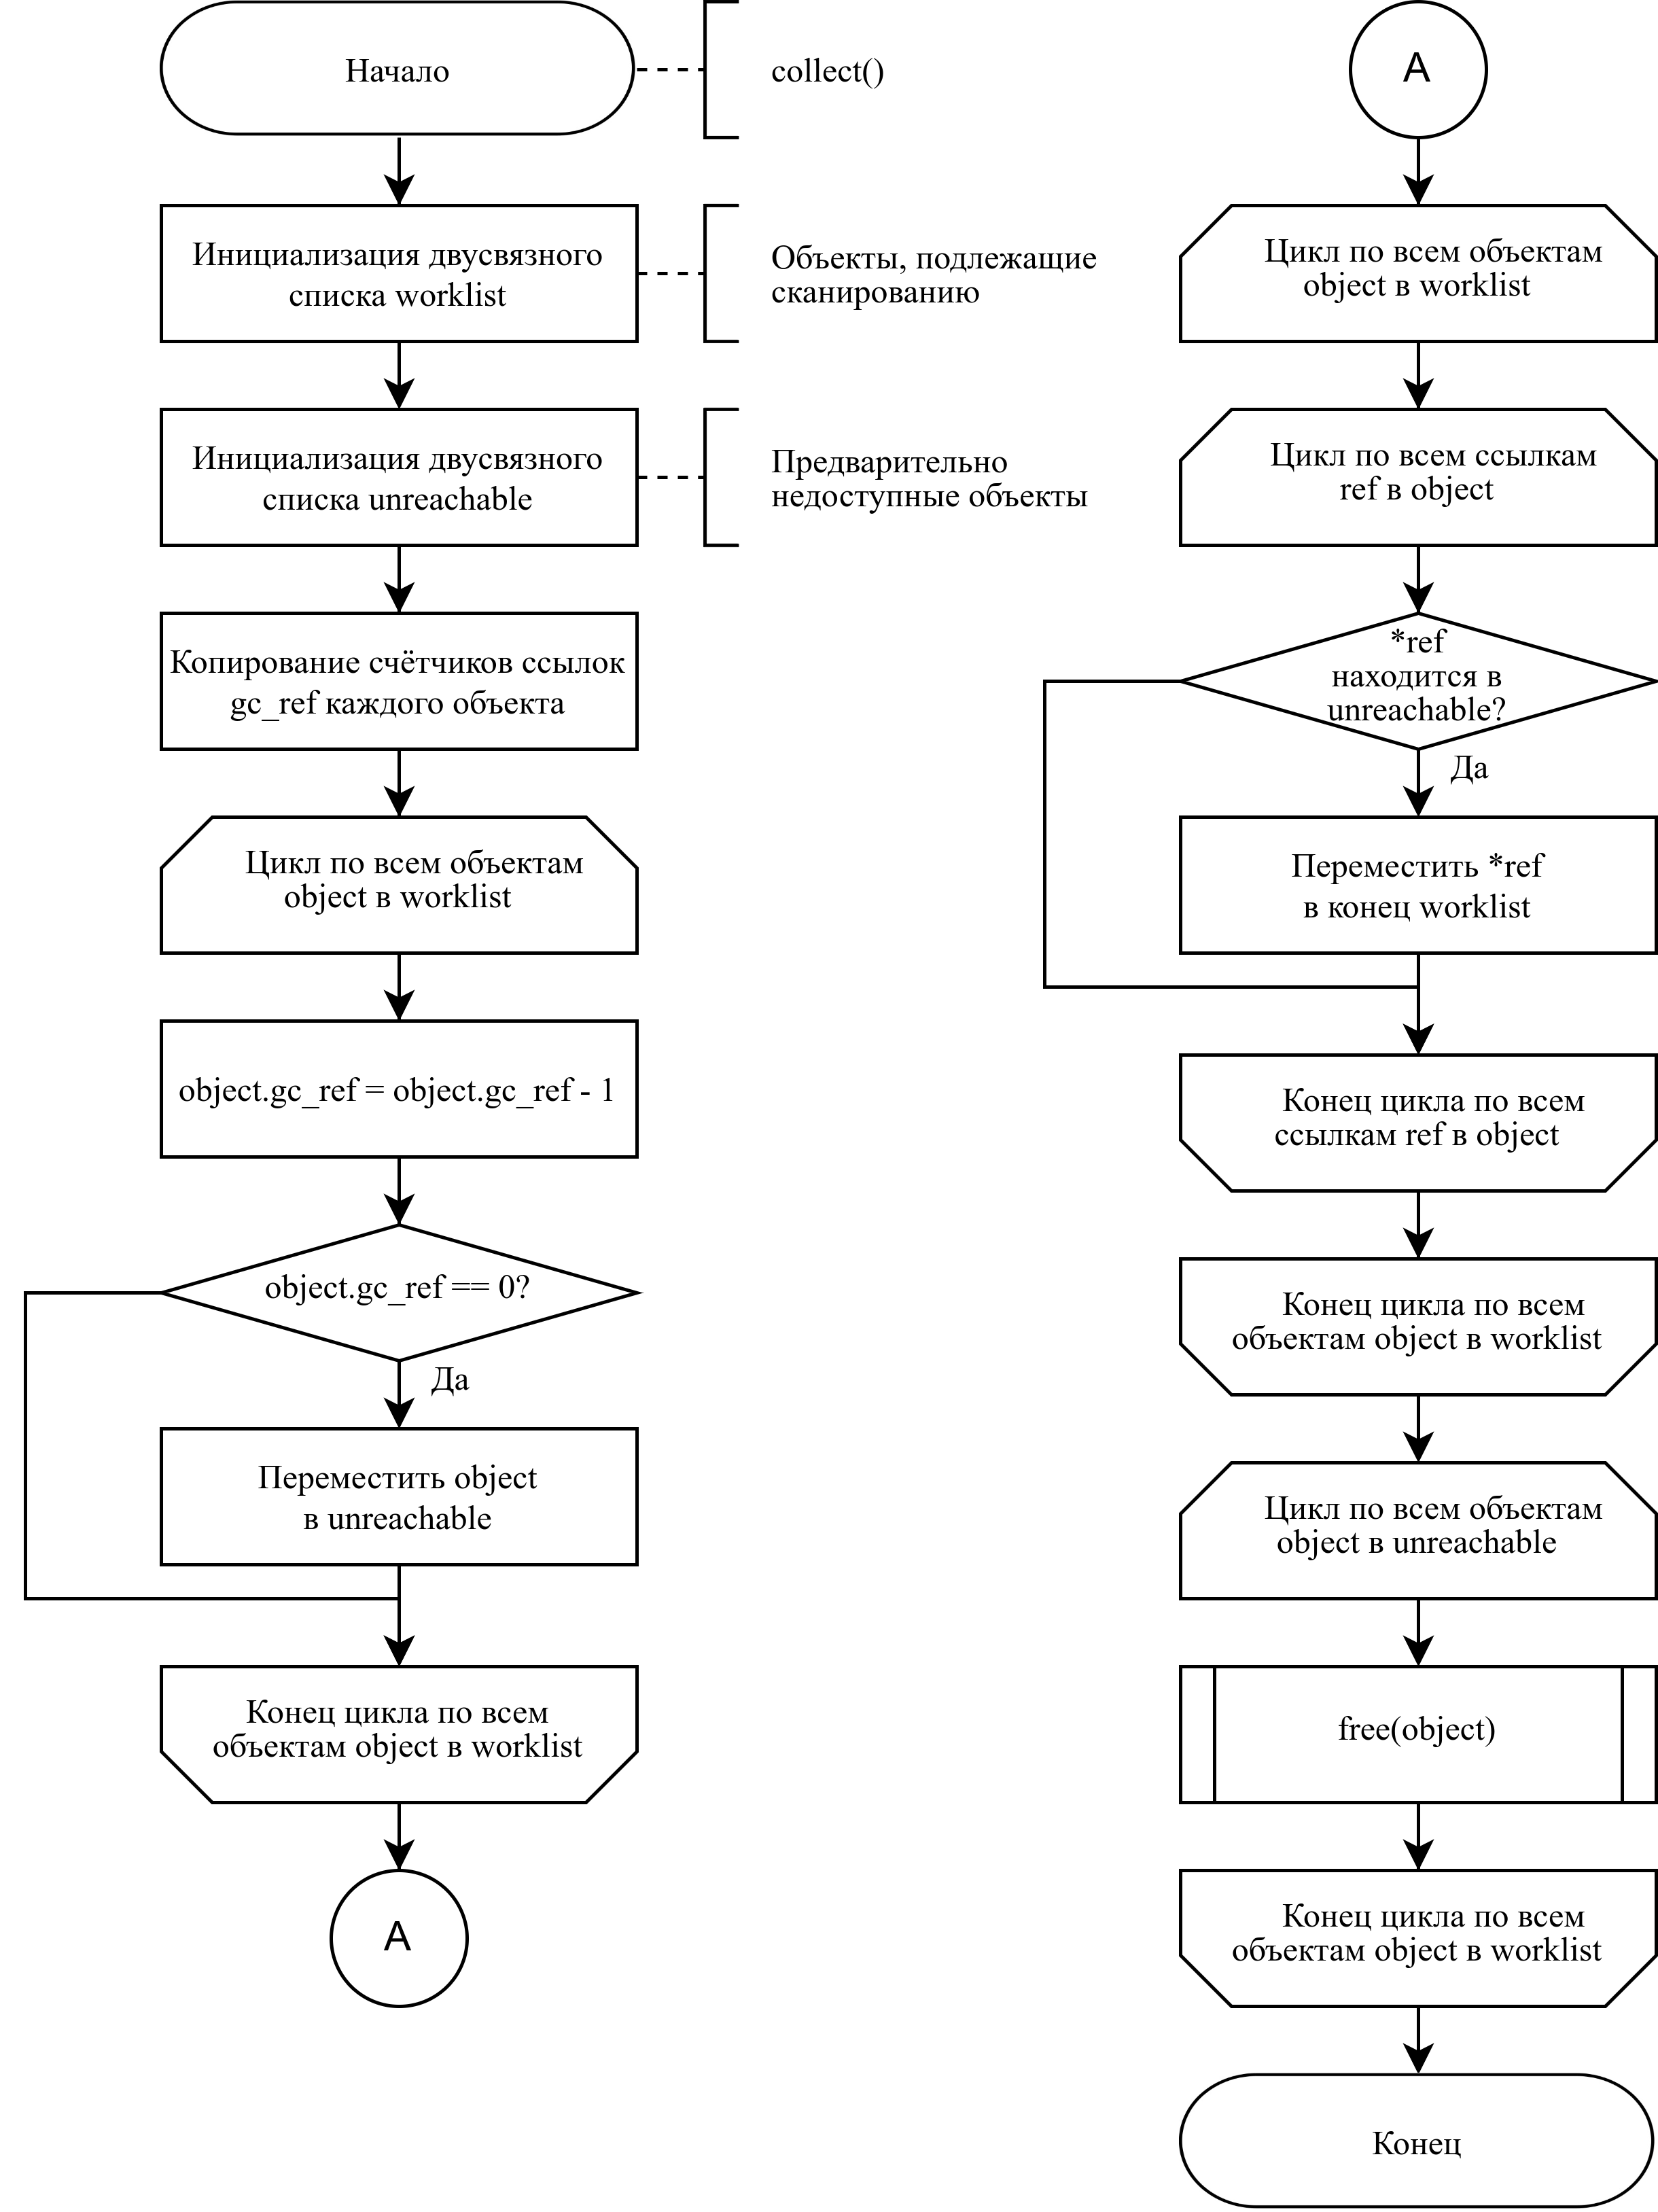
\includegraphics[scale=0.175]{assets/python-gc.png}
	\caption{Схема алгоритма сбора циклических ссылок}
	\label{fig:python-gc}
\end{figure}

\begin{figure}[H]
	\centering
	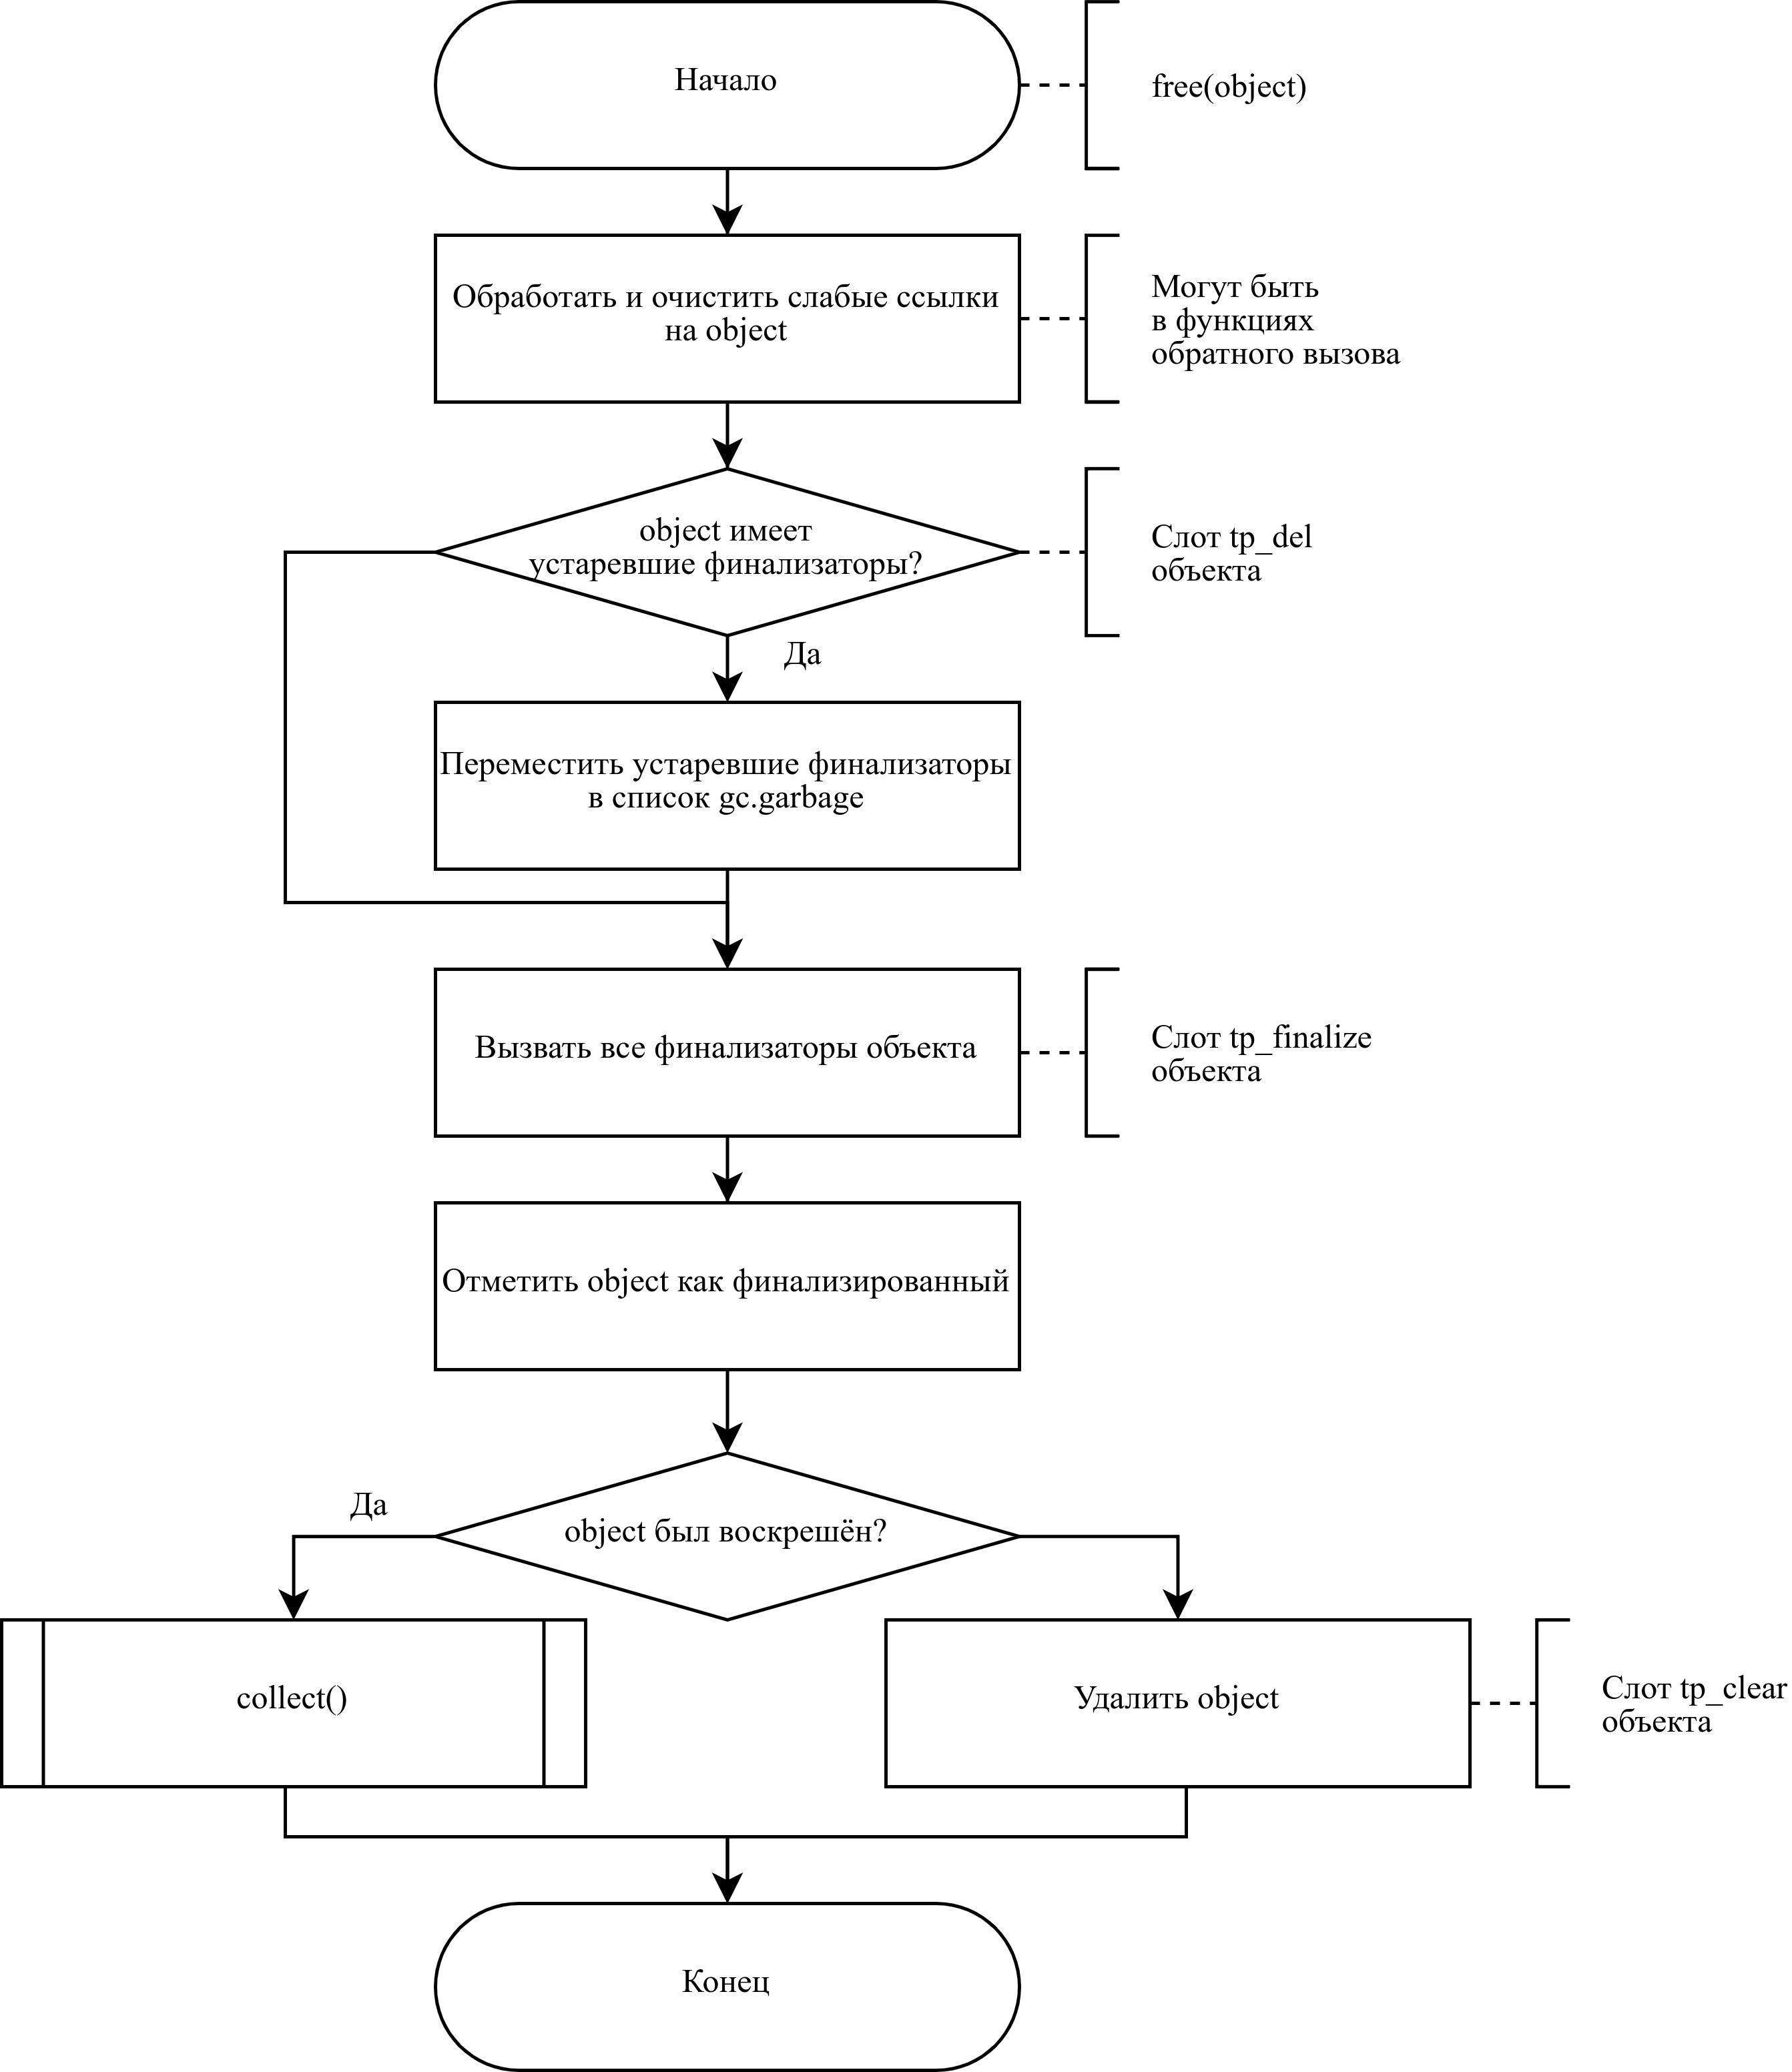
\includegraphics[scale=0.175]{assets/python-free.png}
	\caption{Схема алгоритма освобождения объекта}
	\label{fig:python-free}
\end{figure}



\subsection{Оптимизации}

Для снижения накладных расходов на сборку мусора в языке Python используются следующие оптимизации.

\begin{enumerate}[label*=\arabic*.]
	\item \textbf{Алгоритм поколений} (см. п. \ref{generational}). Для его реализации все объекты-контейнеры разделяются на три пространства (поколения). Каждый новый объект помещается в первое поколение. Алгоритм сбора мусора выполняется только над объектами определённого поколения, и если объект не уничтожается во время обработки своего поколения, он будет перемещён в следующее поколение, где его будут анализировать реже. Если тот же объект не уничтожается после ещё одного цикла сборки мусора, он будет перемещен в последнее поколение, где его будут анализировать реже всего. Чтобы определить момент запуска сбора мусора, сборщик отслеживает количество выделений и освобождений объектов с момента последнего сбора. Когда разность между ними превысит заданный порог (threshold), начнётся сбор. Первоначально исследуется только первое поколение. Если количество его сканирований после последнего анализа первого поколения превысило заданный порог, то также анализируется второе поколение. Последнее поколение сканируется только в том случае, если количество выделений объектов превышает количество освобождений на заданное значение (по умолчанию задано 25\%). \cite{python_gc}
	
	\item \textbf{Повторное использование полей ссылок}. В целях экономии памяти указатели из поля PyGC\_Head каждого объекта используются для нескольких целей. Эта оптимизация носит название <<толстые указатели>> (fat pointers) или <<теговые указатели>> (tag pointers). Так, внутрь указателей помещаются дополнительные данные с учётом следующего свойства адресации памяти: большинство архитектур выравнивают размеры типов данных по определённой величине, зачастую кратной машинному слову. Следовательно, несколько младших бит указателя всегда заполнены нулями и их можно использовать для хранения другой информации, чаще всего в виде битового поля. \cite{python_gc}
	
	\item \textbf{Задержка отслеживания контейнеров}. Определённые типы контейнеров не могут участвовать в цикле ссылок, поэтому сборщик мусора не отслеживает их. Существует два случая, когда отслеживание контейнера откладывается:
	\begin{itemize}[label*=---]
		\item когда контейнер создан;
		\item когда контейнер сканируется сборщиком мусора.
	\end{itemize}
	Как правило, экземпляры простых (атомарных) типов данных не отслеживаются, а экземпляры агрегированных типов (контейнеры, определяемые пользователем объекты и т.д.) отслеживаются. Тем не менее, могут быть предусмотрены некоторые оптимизации для конкретных типов, чтобы снизить влияние сборщика мусора на экземпляры простых типов. Так, кортежи (tuple) и словари (dict), содержащие только неизменяемые объекты (числа, строки, кортежи неизменяемых объектов и т.д.) не отслеживаются сборщиком мусора. \cite{python_gc}
\end{enumerate}

%Рассматриваем только реализацию Cython.
%
%https://docs.python.org/3/c-api/memory.html
%
%https://devguide.python.org/internals/garbage-collector/
%
%https://stackify.com/python-garbage-collection/
%
%https://realpython.com/python-memory-management/https://www.honeybadger.io/blog/memory-management-in-python/
%
%https://medium.com/analytics-vidhya/python-memory-management-8854f4952ba0
%
%https://scoutapm.com/blog/python-garbage-collection
%
%
%
%https://www.javatpoint.com/python-memory-management
%
%https://towardsdatascience.com/memory-management-and-garbage-collection-in-python-c1cb51d1612c
%
%https://rushter.com/blog/python-garbage-collector/
%
%https://scoutapm.com/blog/python-garbage-collection





\section{Java}
\subsection{Управление памятью}
\subsection{Алгоритм работы сборщика мусора}

%https://www.amazon.com/dp/0137142528
%
%https://www.amazon.com/dp/1420082795
%
%
%
%https://en.wikipedia.org/wiki/Garbage-first_collector
%
%
%
%https://docs.oracle.com/cd/E13150_01/jrockit_jvm/jrockit/geninfo/diagnos/garbage_collect.html
%
%https://www.oracle.com/technetwork/java/javase/tech/memorymanagement-whitepaper-1-150020.pdf
%
%https://www.oracle.com/webfolder/technetwork/tutorials/obe/java/gc01/index.html
%
%https://docs.oracle.com/en/java/javase/11/gctuning/garbage-collector-implementation.html
%
%https://docs.oracle.com/javase/8/docs/technotes/guides/vm/gctuning/toc.html
%
%https://docs.oracle.com/javase/specs/jls/se8/html/jls-17.html
%
%https://www.oracle.com/technetwork/tutorials/tutorials-1876574.html
%
%
%
%https://openjdk.org/jeps/0
%
%
%
%https://cyberleninka.ru/article/n/java-garbage-collectors/viewer
%
%
%
%https://www.javatpoint.com/memory-management-in-java
%
%https://opensource.com/article/22/7/garbage-collection-java
%
%https://www.baeldung.com/java-choosing-gc-algorithm
%
%https://www.baeldung.com/jvm-garbage-collectors
%
%https://developers.redhat.com/articles/2021/11/02/how-choose-best-java-garbage-collector
%
%https://developers.redhat.com/articles/2021/08/20/stages-and-levels-java-garbage-collection
%
%https://howtodoinjava.com/java/garbage-collection/revisiting-memory-management-and-garbage-collection-mechanisms-in-java/
%
%https://howtodoinjava.com/java/garbage-collection/all-garbage-collection-algorithms/
%
%
%
%https://assets.ctfassets.net/oxjq45e8ilak/2K7aShH1CgWcUMc4Yqyg0g/b2606c497f7ac0a6bdc36c7c9ba910a1/be-prepared-to-g1-gc-or-evolution-of-the-g1-gc.pdf
%
%
%
%https://habr.com/ru/articles/269621/
%
%https://java-ru-blog.blogspot.com/2020/01/garbage-first-g1-java-vm.html
%
%https://java-online.ru/garbage-collection.xhtml





\section{Javascript}
\subsection{Управление памятью}
\subsection{Алгоритм работы сборщика мусора}

%https://ru.hexlet.io/blog/posts/haskell-yazyk-pozvolyayuschiy-glubzhe-ponyat-programmirovanie-kak-on-ustroen-i-pochemu-ego-vybirayut-razrabotchiki
%
%
%
%https://wiki.haskell.org/GHC/Memory_Management
%
%http://simonmar.github.io/bib/papers/parallel-gc.pdf
%
%https://simonmar.github.io/bib/papers/ExploringBarrierToEntry.pdf
%
%https://www.researchgate.net/publication/221032889_Parallel_generational-copying_garbage_collection_with_a_block-structured_heap
%
%https://stackoverflow.com/questions/36772017/reducing-garbage-collection-pause-time-in-a-haskell-program/36779227
%
%https://well-typed.com/blog/aux/files/nonmoving-gc/design.pdf
%
%https://well-typed.com/blog/2021/03/memory-return/
%
%https://pusher.com/blog/latency-working-set-ghc-gc-pick-two
%
%
%
%https://www.channable.com/tech/lessons-in-managing-haskell-memory
%
%https://pusher.com/blog/making-efficient-use-of-memory-in-haskell/
%
%https://ro-che.info/articles/2017-08-06-manage-allocated-memory-haskell





\section{C\#}
\subsection{Управление памятью}
\subsection{Алгоритм работы сборщика мусора}
%https://learn.microsoft.com/en-us/dotnet/standard/garbage-collection/fundamentals
%
%https://learn.microsoft.com/en-us/dotnet/csharp/advanced-topics/performance/
%
%https://learn.microsoft.com/en-us/dotnet/standard/garbage-collection/
%
%https://www.bytehide.com/blog/garbage-collection-dotnet
%
%https://prographers.com/blog/in-depth-memory-management-in-c
%
%https://habr.com/ru/articles/44208/
%
%https://habr.com/ru/articles/590475/
%
%https://metanit.com/sharp/tutorial/8.1.php
%
%
%
%https://medium.com/c-programming/c-memory-management-part-1-c03741c24e4b
%
%https://medium.com/c-programming/c-memory-management-part-2-finalizer-dispose-d3b3e43c08d1
%
%https://medium.com/c-programming/c-memory-management-part-3-garbage-collection-18faf118cbf1





\section{Golang}

\textbf{Golang} (также \textbf{Go}) \cite{golang} --- компилируемый язык программирования с открытым исходным кодом, разработанный компанией Google. Официально язык был представлен в ноябре 2009 года.

В любой программе на языке Golang присутствует \textbf{среда выполнения} (runtime) \cite{golang_runtime}, то есть код, который выполняется без ведома программиста. Среда выполнения состоит из следующих компонентов.

\begin{enumerate}[label*=\arabic*.]
	\item \textbf{Планировщик} (Sheduler) \cite{golang_scheduler}, отвечающий за управление работой горутин. \textbf{Горутина} --- это легковесный поток, управляемый средой выполнения языка Golang. \cite{golang_goroutine}
	\item \textbf{Аллокатор памяти}.
	\item \textbf{Сборщик мусора}.
\end{enumerate}

\subsection{Выделение памяти}

Первоначально аллокатор памяти языка Golang был основан на \textbf{tcmalloc}~\cite{tcmalloc}, но со временем стал сильно отличаться от него. \cite{golang_malloc} 

Аллокатор работает с наборами страниц (runs of pages). Если размер выделяемого объекта не превышает 32 Кб, то он округляется до одного из 67 \textbf{классов размеров} (size classes) \cite{golang_size_classes}, каждый из которых имеет свой собственный набор свободных объектов соответствующего размера. Любая свободная страница памяти может быть разделена на набор объектов одного класса размера, которыми затем можно управлять с помощью битовой карты свободных областей (free bitmap). \cite{golang_malloc}

Ниже перечислены основные структуры данных, с которыми работает аллокатор памяти в языке Golang. \cite{golang_malloc}

\begin{enumerate}[label*=\arabic*.]
	\item \textbf{fixalloc} \cite{golang_fixalloc} --- аллокатор для объектов фиксированного размера, размещаемых за пределами кучи. Используется для управления хранилищем, которое использует аллокатор.
	\item \textbf{mheap} --- куча, поделённая на страницы размером 8 Кб.
	\item \textbf{mspan} --- набор используемых страниц, управляемых mheap.
	\item \textbf{mcentral} --- хранилище всех mspan заданного класса размера.
	\item \textbf{mcache} --- кеш для каждого ядра процессора, содержащий набор mspan со свободным пространством.
	\item \textbf{mstats} --- статистика распределения памяти.
\end{enumerate}

На рисунке \ref{fig:golang-allocate} показана схема алгоритма выделения памяти.

\begin{figure}[H]
	\centering
	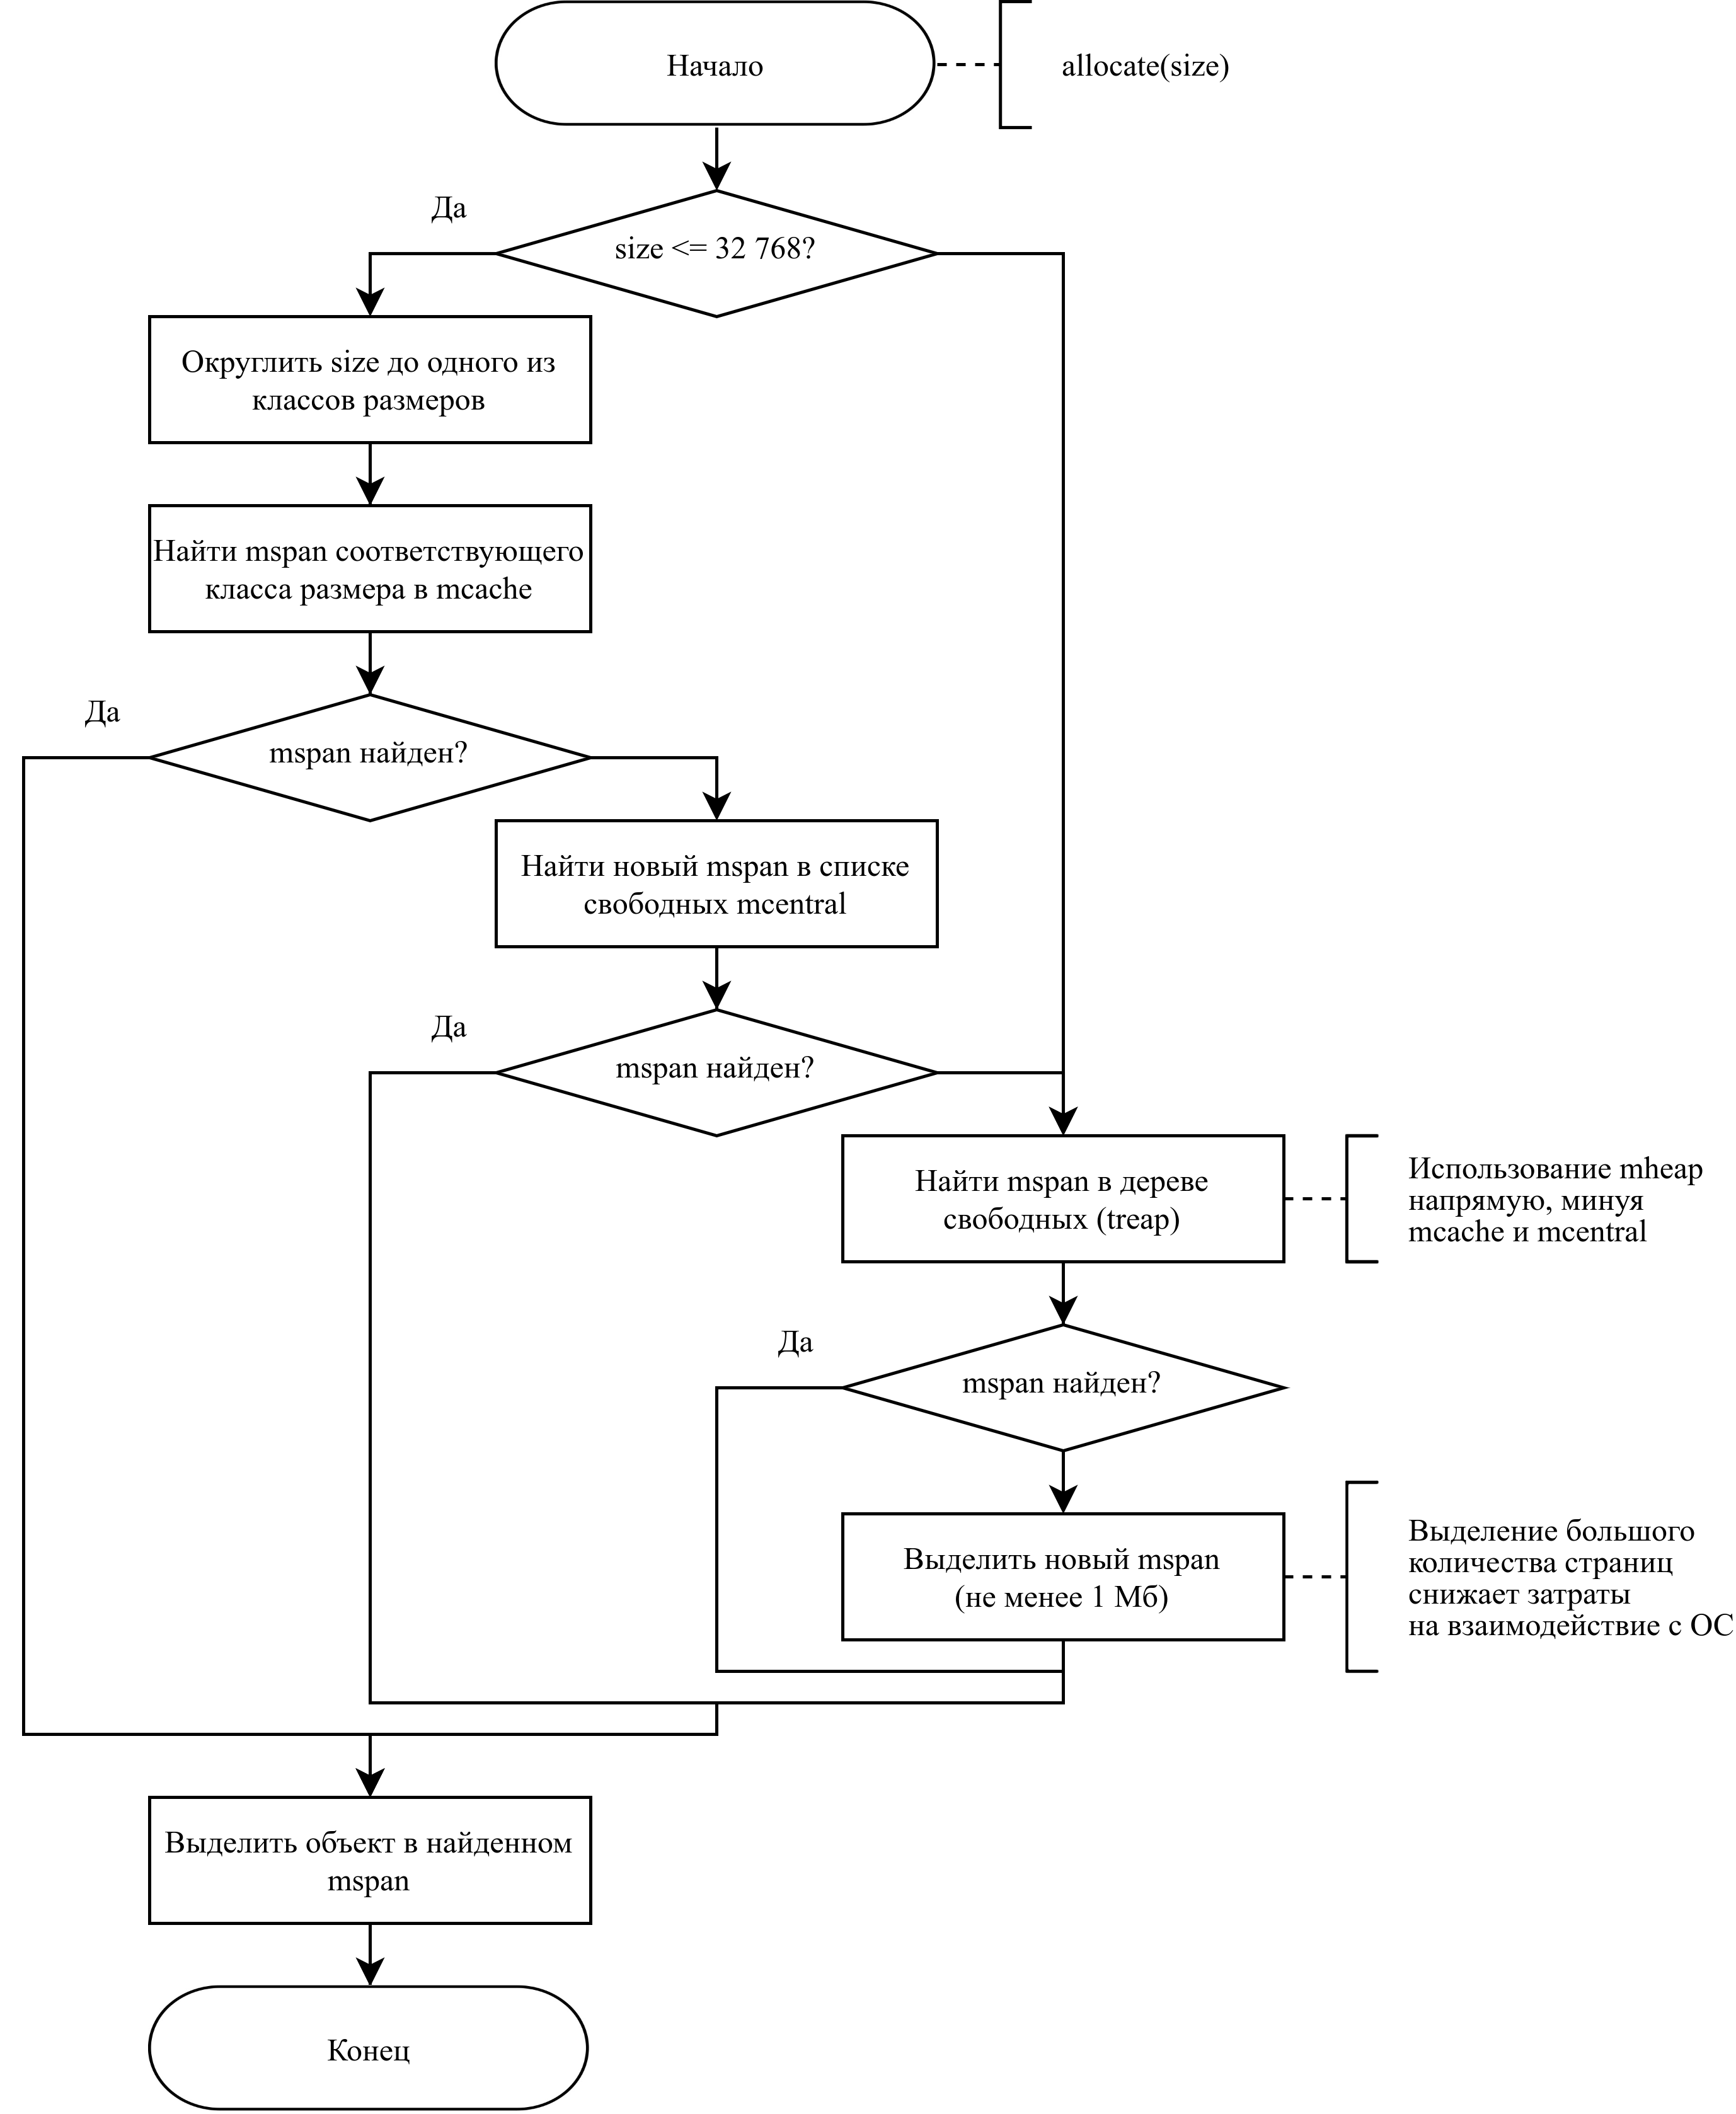
\includegraphics[scale=0.175]{assets/golang-allocate.png}
	\caption{Выделение памяти в куче}
	\label{fig:golang-allocate}
\end{figure}

На рисунке \ref{fig:golang-sweep} показана схема алгоритма освобождения памяти.

\begin{figure}[H]
	\centering
	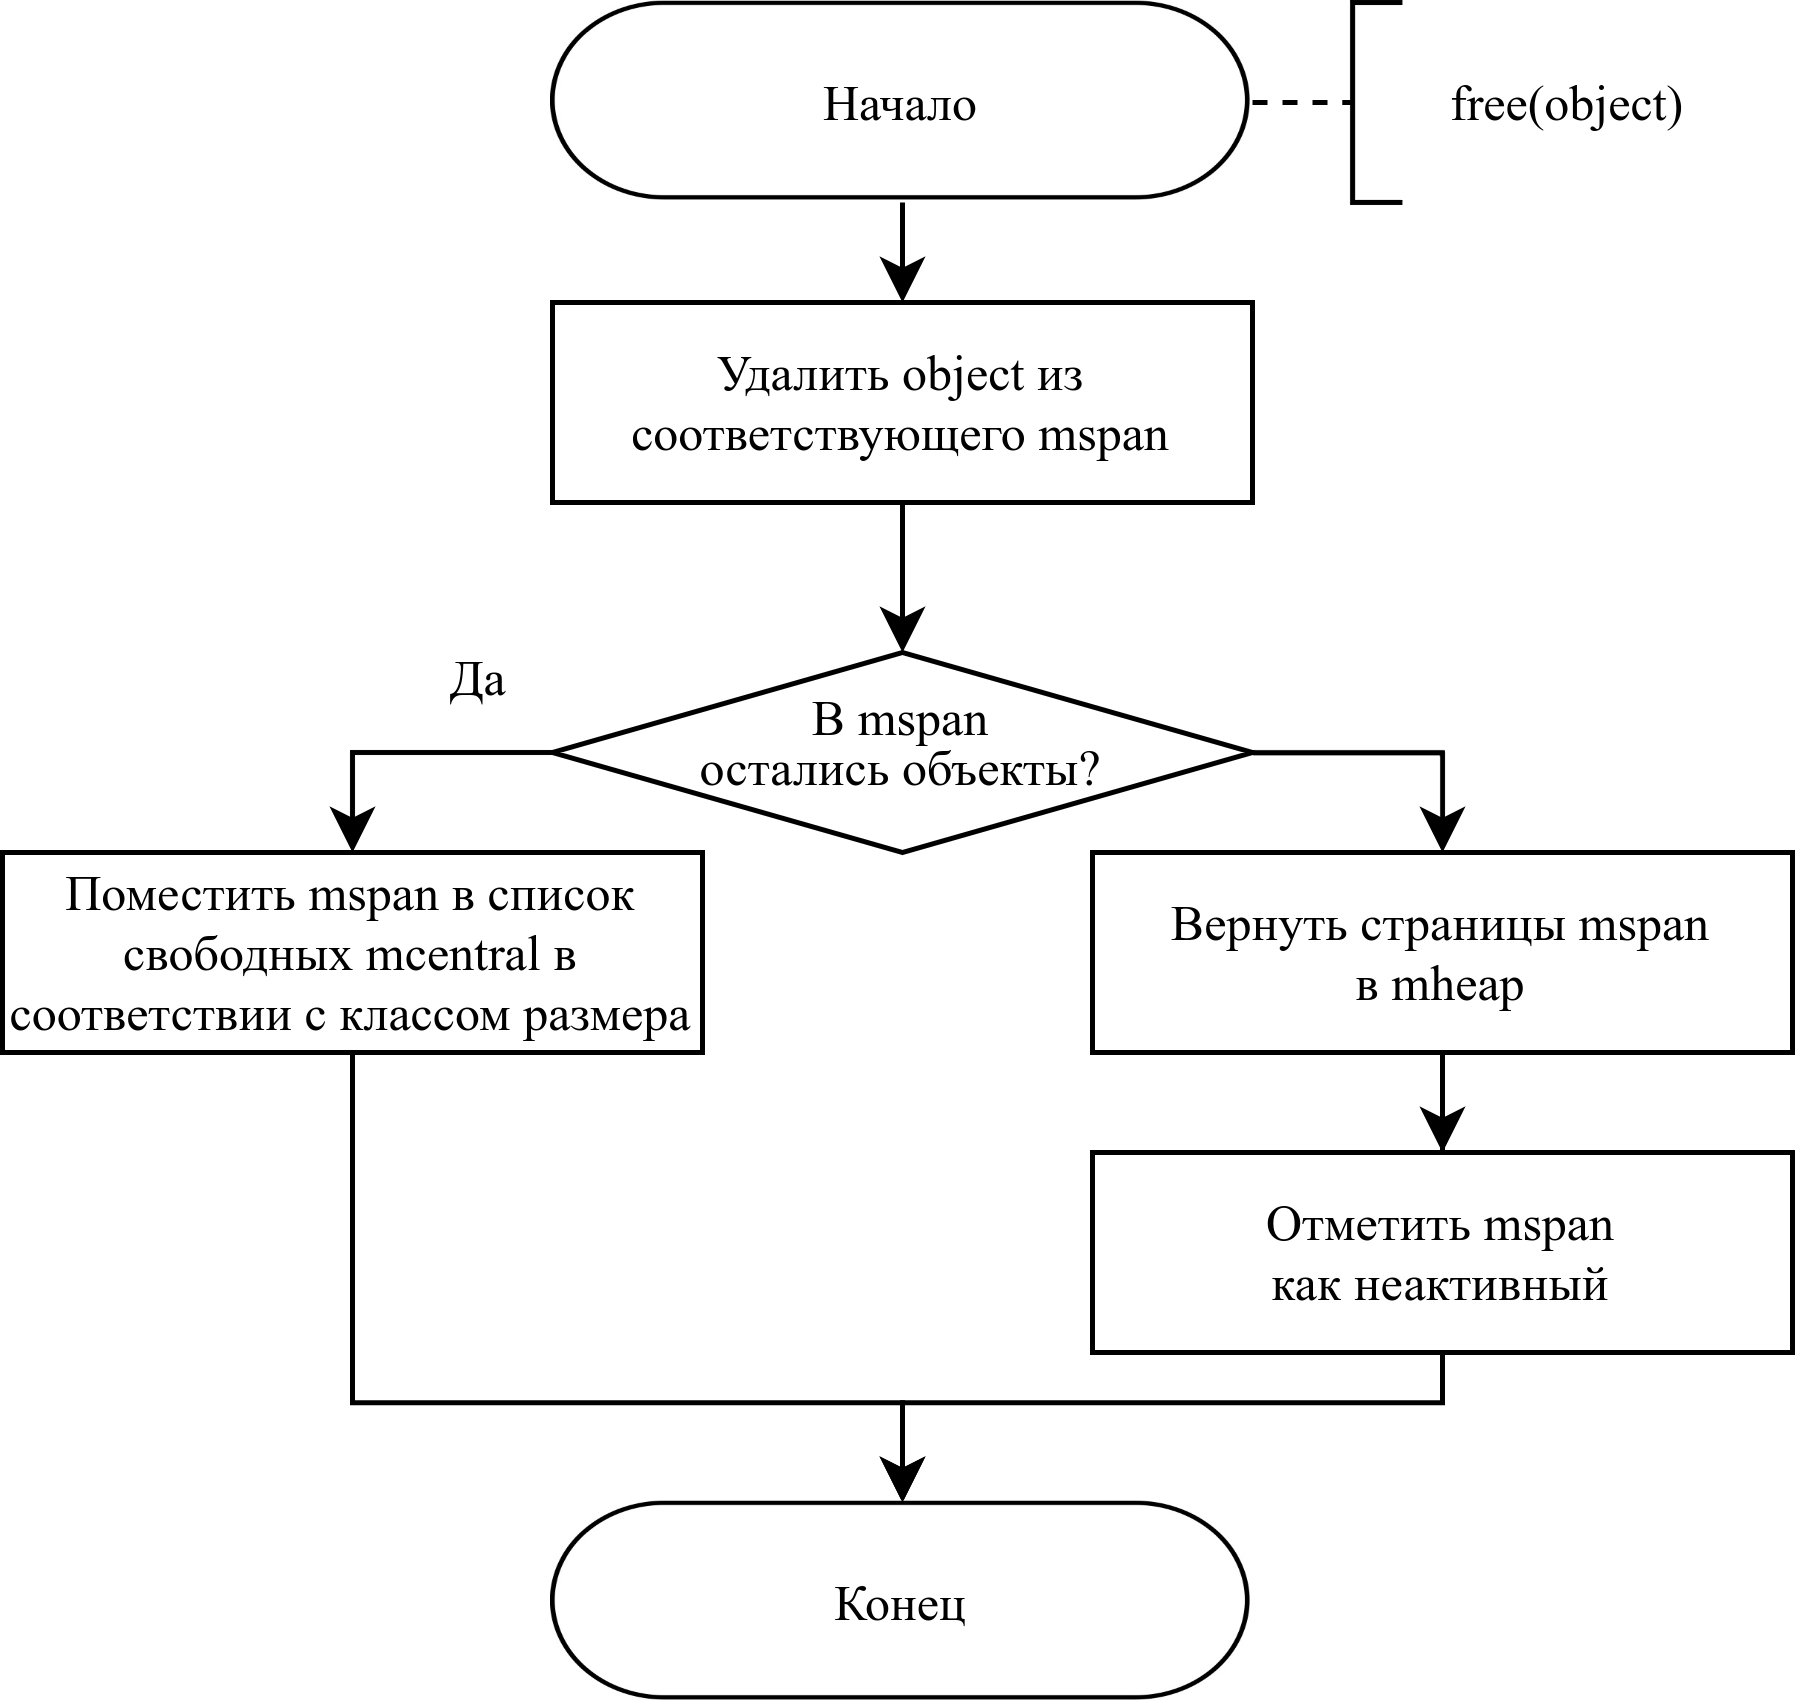
\includegraphics[scale=0.175]{assets/golang-sweep.png}
	\caption{Освобождение памяти в куче}
	\label{fig:golang-sweep}
\end{figure}



\subsection{Структура кучи}

Куча состоит из набора областей, называемых \textbf{аренами} (Arena), размер которых составляет 64 Мб в 64-разрядной версии и 4 Мб в 32-разрядной (heapArenaBytes). Начальный адрес каждой арены также выровнен по размеру арены. \cite{golang_malloc}

С каждой ареной связан объект heapArena \cite{golang_mheap}, который хранит метаданные для этой арены: битовую карту кучи для всех слов (word) в арене и карту span для всех страниц в ней. Объекты heapArena выделяются вне кучи. \cite{golang_malloc}

Структура mheap содержит \textbf{карту арен}, которая охватывает всё доступное адресное пространство программы, поэтому его можно рассматривать как набор арен. Аллокатор старается сохранять арены смежными, чтобы большие span (и, следовательно, большие объекты) могли занимать одновременно несколько арен. \cite{golang_malloc}

Концептуальная схема, отражающая структуру кучи в программе на языке Golang, представлена на рисунке \ref{fig:golang_heap}.

\begin{figure}[H]
	\centering
	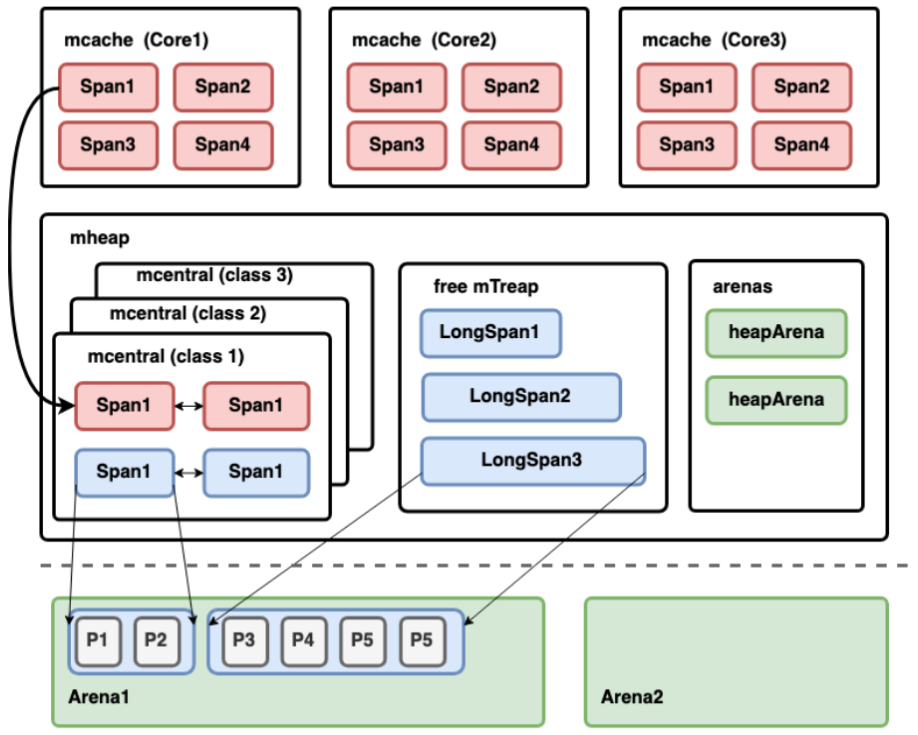
\includegraphics[width=\textwidth]{assets/golang-heap.png}
	\caption{Структура кучи в Golang}
	\label{fig:golang_heap}
\end{figure}



\subsection{Сборка мусора}

В языке Golang для сборки мусора используется алгоритм \textbf{Concurrent Mark-Sweep}, являющийся модификацией алгоритма mark-sweep (см. п. \ref{mark-sweep}), предназначенного для сборки мусора конкурентно с основной программой. \cite{golang_gc}

Сборщик мусора запускается параллельно с потоками основной программы, обладает точностью типов (type accurate, type precise), позволяет нескольким потокам сборки мусора выполняться параллельно. Алгоритм сборки мусора не является уплотняющим и не использует поколения (см. п. \ref{mark-compact} и \ref{generational}). 

Для конкурентной разметки и очистки используются \textbf{барьеры записи} (write barrier), позволяющий избежать ситуации, когда чёрные объекты указывают на белые. Такое может произойти, например, при перемещении указателя в программе до того, как сборщик мусора успел его разметить. В такой ситуации основная программа скрывает объект от сборщика мусора. \cite{golang_gc} Для реализации барьера записи используются операции <<затенения>> (shade), перемещающие указатели программы. Барьер записи затеняет как записываемый указатель, так и записываемое значение при любой записи по указателю \cite{golang_barrier}. 

Ниже представлено высокоуровневое описание основных шагов алгоритма сборки мусора. \cite{golang_gc}

\begin{enumerate}[label*=\arabic*.]
	\item Фаза завершения очистки (sweep termination).
	\begin{enumerate}[label*=\arabic*.]
		\item <<Остановка мира>> (stop the world, см. п. \ref{mark-sweep}), приводящая к тому, что все потоки достигают \textbf{безопасной точки} (GC safe-point).
		\item Очистка всех мусорных mspan. Неочищенные mspan будут только в том случае, если цикл сборки мусора был запущен раньше ожидаемого времени.
	\end{enumerate}

	\item Фаза разметки (mark).
	\begin{enumerate}[label*=\arabic*.]
		\item Включение барьера записи, постановка в очередь заданий по разметке объектов из корневого набора и включение ассистентов (assistants), выполняющих свою работу во время выделения памяти. Никакие объекты не могут быть просканированы до тех пор, пока все потоки не включат барьер записи, что достигается с помощью <<остановки мира>>.
		\item <<Запуск мира>> (start the world). С этого момента работа сборщика мусора выполняется обработчиками разметки (mark workers), запущенными планировщиком, и ассистентами. Выделяемые объекты отмечаются чёрным цветом.
		\item Разметка объектов из корневого набора, включающая в себя сканирование стеков всех горутин, затенение всех глобальных переменных и затенение любых указателей кучи в структурах данных среды выполнения вне кучи. При сканировании стека горутина останавливается, затеняются все указатели, найденные в её стеке, а затем горутина продолжает выполняться.
		\item Очистка рабочей очереди от серых объектов. Каждый серый объект сканируется и отмечается чёрным, затеняя все указатели, найденные в объекте, что, в свою очередь, может привести к добавлению этих указателей в рабочую очередь.
		\item Выполнение алгоритма распределенного завершения (distributed termination algorithm), чтобы определить, когда закончится выполнение заданий разметки объектов из корневого набора или серых объектов.
	\end{enumerate}

	\item Фаза завершения разметки (mark termination).
	\begin{enumerate}[label*=\arabic*.]
		\item <<Остановка мира>>.
		\item Отключение обработчиков и ассистентов.
		\item Очистка, включающая сброс кешей mcache.
	\end{enumerate}

	\item Фаза очистки (sweep).
	\begin{enumerate}[label*=\arabic*.]
		\item Отключение барьера записи.
		\item <<Запуск мира>>. С этого момента выделяемые объекты становятся белыми. Также при необходимости аллокатор может очищать mspan перед использованием.
		\item Выполнение параллельной очистки в фоновом режиме и во время выделения памяти.
	\end{enumerate}
\end{enumerate}

Чтобы предотвратить длительные паузы при сканировании больших объектов и улучшить параллелизм, сборщик мусора разбивает задания сканирования объектов размером более maxObletBytes на \textbf{<<облеты>>}, размер которых не превышает maxObletBytes. Когда при сканировании обнаруживается начало большого объекта, сборщик сканирует только первый фрагмент, а остальные фрагменты помещает в очередь как новые задания сканирования. \cite{golang_gc}



\subsection{Настройка сборщика мусора}

Следующая сборка мусора выполняется после того, как был выделен дополнительный объём памяти, пропорциональный тому который был зафиксирован при предыдущем запуске сборки мусора. Данная пропорция контролируется переменной среды \textbf{GOGC} (по умолчанию  имеет значение 100). Если GOGC=100 и программа использует 4 Мб памяти, следующий цикл сборки мусора запустится тогда, когда объём используемой памяти достигнет 8 Мб. Такая настройка позволяет сохранить линейную зависимость накладных расходов на сборку мусора от накладных расходов на выделение памяти. Настройка GOGC просто изменяет линейную константу. \cite{golang_gc}

По сути GOGC определяет компромисс между накладными расходами памяти и процессорного времени. Определяется целевой размер кучи после каждого цикла сборки мусора, а также целевое значение общего размера кучи для запуска следующего цикла. Целевой размер кучи определяется следующим образом. \cite{golang_gc_guide}

\begin{equation}
	Target\ heap = Live\ heap + (Live\ heap + GC\ roots) * GOGC / 100
\end{equation}

Стоит заметить, что данная настройка не учитывает то, что доступная программе память ограничена. В версии Golang 1.19 было добавлено ограничение, которое устанавливает максимальный общий объем памяти (\textbf{GOMEMLIMIT}), который может использовать среда выполнения Golang. \cite{golang_1_19} \cite{golang_proposal_limit}

Поскольку сборщик мусора имеет явный контроль над тем, сколько памяти кучи используется программой, он устанавливает общий размер кучи на основе этого ограничения памяти и того, сколько другой памяти использует среда выполнения Golang. Когда размер используемой памяти достигает пикового значения, определенного GOGC, сборщик мусора запускается чаще, чтобы поддерживать его в пределах лимита. \cite{golang_gc_guide}

Стоить заметить, что даже когда GOGC отключен, ограничение памяти всё равно соблюдается. Это позволяет достичь максимальной экономии ресурсов, поскольку устанавливается мини \cite{golang_gc_guide}мальная частота запуска сборщика мусора, необходимая для поддержания ограничения памяти.

Несмотря на то, что ограничение памяти, очевидно, является мощным инструментом, его использование не обходится без накладных расходов и, конечно же, не отменяет полезность GOGC. \cite{golang_gc_guide}

Такая ситуация, когда программа не может выполняться из-за постоянных циклов сборки мусора, называется \textbf{перегрузкой}. Во многих случаях неопределённая остановка хуже, чем нехватка памяти, которая обычно приводит к гораздо более быстрому сбою. По этой причине ограничение памяти в Golang определяется как \textbf{мягкое} (soft memory limit) \cite{golang_proposal_limit}. Среда выполнения Go не дает никаких гарантий, что она сохранит заданный лимит памяти при любых обстоятельствах, а только обещает некоторое разумное количество усилий. Это ослабление ограничения памяти имеет решающее значение для предотвращения зависаний, поскольку оно позволяет аллокатору превысить предел, чтобы не тратить слишком много времени на сборку мусора. \cite{golang_gc_guide}

В языке Golang мягкое ограничение памяти реализовано следующим образом: сборщик мусора устанавливает верхний предел количества процессорного времени, которое он может использовать в течение некоторого временного промежутка (окна, frame). В настоящее время этот предел установлен примерно на уровне 50\%. В случае неправильной настройки лимита памяти, когда по ошибке он был установлен слишком низким, программа замедлится максимум в 2 раза, поскольку GC не может отнять у неё более 50\% процессорного времени. \cite{golang_gc_guide}


\subsection{Арены памяти}

В версии Golang 1.20 появилось экспериментальное решение для управления памятью, которое позволяет совместить безопасное выделение динамической памяти и уменьшение влияния среды выполнения языка, включающей интегрированный менеджер памяти, на производительность приложения.

% С точки зрения распределения памяти работа с ареной похожа на выделение одной области памяти (который может увеличиваться в размере) и при освобождении арены все выделенные в ней объекты становятся недоступными.

Пакет arena предоставляет возможность выделения памяти в программах на языке Golang и освобождать её вручную, причем безопасно и одновременно. Цель этой функциональности --- повышение эффективности программ: освобождение памяти вручную откладывает следующий цикл сборки мусора. В свою очередь, снижение частоты циклов означает уменьшение накладных расходов на сборку мусора. \cite{golang_arena_cource}

Большая часть описанной функциональности рассматриваемого пакета реализована в типе Arena, который является абстракцией относительно большого объёма памяти, выделенного в куче. Наиболее эффективное использование Arena достигается при хранении в них некоторого множества объектов программы, занимающих около 1 Мб памяти. \cite{golang_arena_cource} \cite{golang_arena_proposal}

Стоит заметить, что при использовании этой ограниченной формы ручного выделения памяти возможны ошибки типа <<use-after-free>> (использование после освобождения). Пакет Arena ограничивает влияние этих ошибок, предотвращая повторное использование освобождённых областей памяти до тех пор, пока сборщик мусора не сможет убедиться в том, что это безопасно. Как правило, ошибка <<use-after-free>> приводит к сбою и получению сообщения об ошибке, но пакет Arena оставляет за собой право не вызывать сбой программы при использовании освобождённой памяти. Это означает, что реализация данного пакета допускает выделение памяти так, как это обычно делает среда выполнения, оставляя за собой право иногда делать это для некоторых объектов программы.~\cite{golang_arena_cource}

Повышение производительности программы, использующей выделение памяти на аренах, можно ожидать в тех случаях, когда приложение интенсивно выделяет память (например, при работе с ссылочными структурами данных, такими как двоичные деревья), но при этом предполагается, что выделенные структуры данных являются относительно долгоживущими и существуют до момента освобождения арены целиком (сборщик мусора для арены не применяется и выделенные на ней объекты не освобождаются автоматически). 


%Мои конспекты в Obsidian
%
%Лекция
%
%https://habr.com/ru/companies/oleg-bunin/articles/676332/
%
%https://go101.org/article/memory-block.html
%
%https://go.dev/ref/mem
%
%https://go.dev/doc/gc-guide
%
%https://github.com/golang/proposal/blob/master/design/48409-soft-memory-limit.md (ALSO FOR JAVA)
%
%https://github.com/golang/go/issues/51317
%
%https://backendinterview.ru/goLang/memory.html
%
%
%
%https://medium.com/safetycultureengineering/an-overview-of-memory-management-in-go-9a72ec7c76a8
%https://medium.com/@ali.can/memory-optimization-in-go-23a56544ccc0
